% ============================================================
%  INTERCICLO REPORT — Stereo Vision and Augmented Reality
%  Universidad Politécnica Salesiana · Visión Artificial G8
%  Author: Michael Lata · Period: April–August 2026
% ============================================================
\documentclass[12pt, a4paper]{article}

% ── Encoding and language ─────────────────────────────────
\usepackage[utf8]{inputenc}
\usepackage[T1]{fontenc}
\usepackage[english]{babel}

% ── Typography ────────────────────────────────────────────
\usepackage{lmodern}
\usepackage{microtype}

% ── Page layout ───────────────────────────────────────────
\usepackage[top=2.5cm, bottom=2.5cm, left=3cm, right=2.5cm]{geometry}
\usepackage{fancyhdr}
\pagestyle{fancy}
\fancyhf{}
\rhead{\small Stereo Vision · Mid-Semester 2026}
\lhead{\small Universidad Polit\'ecnica Salesiana}
\cfoot{\thepage}
\renewcommand{\headrulewidth}{0.4pt}

% ── Mathematics ───────────────────────────────────────────
\usepackage{amsmath, amssymb}

% ── Plots and diagrams ────────────────────────────────────
\usepackage{pgfplots}
\pgfplotsset{compat=1.18}
\usepackage{tikz}
\usetikzlibrary{shapes.geometric, arrows.meta, positioning, fit,
                backgrounds, calc, decorations.pathreplacing}

% ── Tables ────────────────────────────────────────────────
\usepackage{booktabs}
\usepackage{multirow}
\usepackage{array}

% ── Source code ───────────────────────────────────────────
\usepackage{listings}
\usepackage{xcolor}

\definecolor{codegreen}{rgb}{0.13,0.54,0.13}
\definecolor{codegray}{rgb}{0.5,0.5,0.5}
\definecolor{codeblue}{rgb}{0.00,0.20,0.60}
\definecolor{backcolour}{rgb}{0.97,0.97,0.97}

\lstdefinestyle{cppstyle}{
  backgroundcolor=\color{backcolour},
  commentstyle=\color{codegreen}\itshape,
  keywordstyle=\color{codeblue}\bfseries,
  numberstyle=\tiny\color{codegray},
  stringstyle=\color{orange},
  basicstyle=\ttfamily\footnotesize,
  breaklines=true,
  captionpos=b,
  keepspaces=true,
  numbers=left,
  numbersep=5pt,
  showspaces=false,
  tabsize=2,
  language=C++,
  literate=%
    {á}{{\'{a}}}1 {é}{{\'{e}}}1 {í}{{\'{i}}}1 {ó}{{\'{o}}}1 {ú}{{\'{u}}}1
    {ñ}{{\~{n}}}1 {ü}{{\"u}}1 {Á}{{\'{A}}}1 {É}{{\'{E}}}1 {Í}{{\'{I}}}1
    {Ó}{{\'{O}}}1 {Ú}{{\'{U}}}1 {Ñ}{{\~{N}}}1
    {—}{{---}}1 {·}{{$\cdot$}}1
}

% ── Figures ───────────────────────────────────────────────
\usepackage{graphicx}
\usepackage{subcaption}
\usepackage{float}

% ── Institutional colors ──────────────────────────────────
\definecolor{salesiana}{RGB}{0, 84, 166}
\definecolor{accentgreen}{RGB}{34, 139, 34}
\definecolor{accentorange}{RGB}{204, 85, 0}

% ── Section format ────────────────────────────────────────
\usepackage{titlesec}
\titleformat{\section}{\large\bfseries\color{salesiana}}{\thesection.}{0.5em}{}
\titleformat{\subsection}{\normalsize\bfseries\color{salesiana!80!black}}{\thesubsection.}{0.5em}{}

% ── Hyperlinks ────────────────────────────────────────────
\usepackage{hyperref}
\hypersetup{
  colorlinks=true,
  linkcolor=salesiana,
  citecolor=accentgreen,
  urlcolor=accentorange,
}

% ── References ────────────────────────────────────────────
\usepackage[numbers, sort&compress]{natbib}
\bibliographystyle{IEEEtranN}

% ── Utilities ─────────────────────────────────────────────
\usepackage{enumitem}
\usepackage{caption}
\captionsetup{font=small, labelfont=bf}

% ============================================================
\begin{document}

% ── Cover page (Spanish, institutional — unchanged) ───────
\begin{titlepage}
\centering
\vspace*{0.8cm}
{\color{salesiana}\rule{\linewidth}{2pt}}\\[0.35cm]
{\Large\bfseries UNIVERSIDAD POLIT\'ECNICA SALESIANA}\\[0.15cm]
{\normalsize CARRERA DE INGENIER\'IA EN CIENCIAS DE LA COMPUTACI\'ON}\\[0.2cm]
{\color{salesiana}\rule{\linewidth}{1pt}}

\vspace{2.2cm}

\parbox{0.80\textwidth}{\centering\LARGE\bfseries\color{salesiana}
  Sistema de Estimaci\'on de Profundidad Estereoscp\'opica
  en Tiempo Real con Realidad Aumentada\\[0.3cm]
  \large mediante Microcontroladores ESP32-CAM
}

\vspace{1.4cm}

{\large\bfseries Informe Interciclo --- Visi\'on Artificial (G8)}\\[0.2cm]
{\normalsize Proyecto Integrador Final --- Parte I}

\vspace{1.6cm}

\begin{tabular}{@{}ll@{}}
\textbf{Autores:}    & Michael Lata $\cdot$ Jordy Romero \\[0.25cm]
\textbf{Docente:}    & Vladimir Robles Bykbaev \\[0.25cm]
\textbf{Asignatura:} & Visi\'on Artificial \\[0.25cm]
\textbf{Per\'iodo:}  & Abril -- Agosto 2026 \\[0.25cm]
\textbf{Fecha:}      & 8 de junio de 2026 \\
\end{tabular}

\vfill
{\color{salesiana}\rule{\linewidth}{2pt}}
\end{titlepage}

% ── Abstract ─────────────────────────────────────────────
\begin{abstract}
This report documents the design and implementation of a real-time stereoscopic
vision system capable of estimating the depth of objects in a scene and overlaying
dynamic Augmented Reality (AR) effects that respond to the measured distance.
The system integrates two ESP32-CAM AI~Thinker microcontrollers, whose firmware was
tuned to guarantee photometric parity between both cameras, with a desktop application
developed in C++17 with OpenCV~4.x under a Model-View-Controller (MVC) architecture.

The processing pipeline spans from concurrent frame acquisition via HTTP with
\texttt{libcurl}, through stereoscopic calibration, preprocessing with adaptive
histogram equalization (CLAHE), disparity estimation using the Semi-Global Block
Matching (SGBM) algorithm, Weighted Least Squares (WLS) post-processing filtering,
and 3D reprojection with the perspective matrix $\mathbf{Q}$, up to temporal
stabilization of the depth coordinate $Z$ through a scalar Kalman filter.

Quantitative evaluations over 50 samples per distance show a mean absolute error
of $0.48$\,cm at 30\,cm, $0.37$\,cm at 60\,cm, and $0.52$\,cm at 90\,cm; with
standard deviations of $1.50$, $0.73$, and $0.44$\,cm respectively, all within the
$\pm3$\,cm threshold required by the rubric.
The implemented AR effect---sinusoidal pixel distortion with cubic decay $1/Z^3$
plus a pulsing energy aura---reacts in amplitude, speed, and color to the
real-time calculated distance.
\end{abstract}

\clearpage
\tableofcontents
\clearpage

% ============================================================
\section{Introduction}
% ============================================================

Estimating the three-dimensional structure of a scene from flat images is one of
the most studied problems in computer vision.
Stereoscopic vision---the computational analogue of human binocular perception---
addresses this problem by computing the apparent displacement (disparity) of the
same physical point between two rectified images captured from two slightly
different viewpoints, and then converting that disparity into metric depth $Z$
using basic projective geometry \cite{hartley2003multiple}.

In practice, implementing a stereo system on low-cost hardware introduces a series
of non-trivial technical challenges:

\begin{itemize}[leftmargin=2em]
  \item \textbf{Hardware synchronization.} Each camera operates its own image sensor
        with its own clock and automatic exposure controllers. Unsynchronized exposure
        or gain values produce luminance differences between the left and right images
        that degrade the accuracy of block matching.
  \item \textbf{Network jitter.} When both cameras transmit over WiFi, packet arrival
        times vary, so the two frames of a stereo pair may correspond to different
        instants. This temporal parallax corrupts the disparity map for moving objects.
  \item \textbf{Disparity granularity at low resolution.} The depth resolution of a
        stereo system is $\Delta Z = Z^2 / (f \cdot B)$, where $f$ is the focal length
        in pixels and $B$ is the baseline. With short focal lengths and compact
        baselines---typical of ESP32-CAM setups---each additional centimeter of real
        depth can correspond to less than one pixel change in disparity.
  \item \textbf{Real-time constraint.} Disparity algorithms such as SGBM are
        computationally expensive. Achieving interactive frame rates on a personal
        computer while running AR rendering requires careful pipeline design.
\end{itemize}

This report describes how each of these challenges was addressed through a combination
of firmware-level optimizations on the microcontrollers and a layered C++ software
pipeline. The design is also validated against the mid-semester rubric criteria:
capture architecture, disparity map quality, distance accuracy and stability, and
originality of the AR effect.

% ============================================================
\section{Problem Statement}
% ============================================================

The central problem is: \textit{given a pair of low-cost WiFi cameras in a fixed but
unknown relative position, estimate the metric depth of an object located at the
center of the binocular visual field, and communicate that depth to the user in real
time via a numerical on-screen indicator and a dynamic visual effect.}

The two specific technical constraints that make the problem non-trivial are:

\begin{enumerate}
  \item \textbf{Photometric instability.} The OV2640 sensor integrated in the
        ESP32-CAM AI~Thinker module has automatic exposure, gain, and white-balance
        controllers that operate asynchronously in each camera. Without intervention,
        the two images of a stereo pair exhibit different brightness levels and color
        tones, making the block-matching search performed by SGBM unreliable.
  \item \textbf{Noise in depth readings.} Even after high-quality calibration and
        disparity filtering, the raw per-frame depth reading oscillates due to sensor
        noise, JPEG compression artifacts, and sub-pixel disparity quantization.
        A direct reading shown to the user would be visually unstable, alternating,
        for example, between 58\,cm and 72\,cm for an object located at 65\,cm.
\end{enumerate}

The solution must also include an original visual AR effect---implemented via direct
pixel manipulation---whose geometry and intensity react measurably to the computed
depth value.

% ============================================================
\section{System Architecture}
% ============================================================

\subsection{General Design: MVC in C++}

The application follows the \textbf{Model-View-Controller (MVC)} architectural
pattern \cite{gamma1994design}, which cleanly separates three responsibilities:

\begin{itemize}[leftmargin=2em]
  \item \textbf{Model} --- data and algorithms independent of visualization:
        \texttt{CameraSource} (frame acquisition), \texttt{StereoCalibration}
        (matrix loading and storage), \texttt{StereoProcessor}
        (CLAHE + SGBM + WLS + 3D reprojection), and \texttt{KalmanDepth}
        (temporal depth filter).
  \item \textbf{View} --- the rendering layer: \texttt{ARRenderer}
        (pixel vignette and energy aura) and \texttt{DisplayManager}
        (three OpenCV windows with overlaid HUD).
  \item \textbf{Controller} --- \texttt{StereoController}, the main loop that reads
        frames from the model, processes them, and delivers results to the view,
        while also managing user interaction (keyboard and mouse).
\end{itemize}

Figure~\ref{fig:pipeline} shows the complete processing pipeline together with the
MVC layer that owns each stage.

% ── Pipeline diagram ─────────────────────────────────────
\begin{figure}[htbp]
\centering
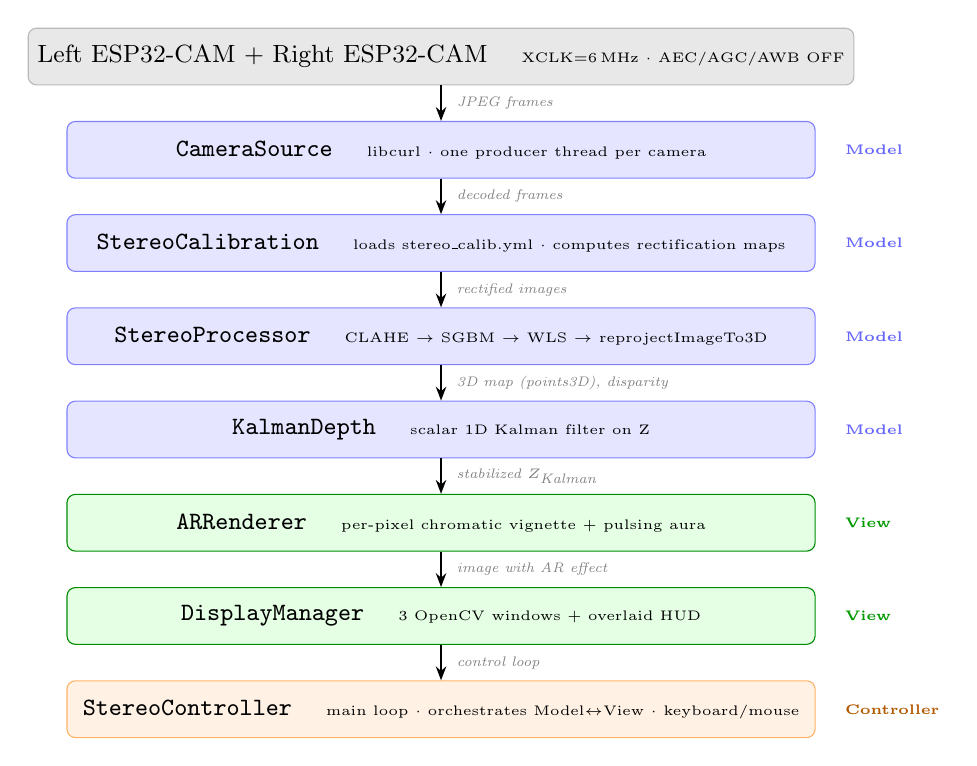
\begin{tikzpicture}[
    node distance = 0.45cm,
    W/.style  = {rectangle, rounded corners=3pt, minimum width=9.5cm,
                 minimum height=0.72cm, align=center, font=\small},
    hw/.style    = {W, fill=gray!18,   draw=gray!55},
    model/.style = {W, fill=blue!10,   draw=blue!50},
    view/.style  = {W, fill=green!10,  draw=green!55!black},
    ctrl/.style  = {W, fill=orange!10, draw=orange!60},
    arr/.style   = {-{Stealth[length=5pt]}, thick},
    lbl/.style   = {font=\tiny\itshape, text=gray, right=2pt}
]

\node[hw]    (hw1)  {Left ESP32-CAM + Right ESP32-CAM \quad{\tiny XCLK=6\,MHz $\cdot$ AEC/AGC/AWB OFF}};
\node[model, below=0.45cm of hw1]  (cam)   {\texttt{CameraSource} \quad{\tiny libcurl $\cdot$ one producer thread per camera}};
\node[model, below=0.45cm of cam]  (calib) {\texttt{StereoCalibration} \quad{\tiny loads stereo\_calib.yml $\cdot$ computes rectification maps}};
\node[model, below=0.45cm of calib](proc)  {\texttt{StereoProcessor} \quad{\tiny CLAHE $\to$ SGBM $\to$ WLS $\to$ reprojectImageTo3D}};
\node[model, below=0.45cm of proc] (kal)   {\texttt{KalmanDepth} \quad{\tiny scalar 1D Kalman filter on Z}};
\node[view,  below=0.45cm of kal]  (ar)    {\texttt{ARRenderer} \quad{\tiny per-pixel chromatic vignette + pulsing aura}};
\node[view,  below=0.45cm of ar]   (disp)  {\texttt{DisplayManager} \quad{\tiny 3 OpenCV windows + overlaid HUD}};
\node[ctrl,  below=0.45cm of disp] (ctrl)  {\texttt{StereoController} \quad{\tiny main loop $\cdot$ orchestrates Model$\leftrightarrow$View $\cdot$ keyboard/mouse}};

\draw[arr] (hw1)  -- node[lbl]{JPEG frames} (cam);
\draw[arr] (cam)  -- node[lbl]{decoded frames} (calib);
\draw[arr] (calib)-- node[lbl]{rectified images} (proc);
\draw[arr] (proc) -- node[lbl]{3D map (points3D), disparity} (kal);
\draw[arr] (kal)  -- node[lbl]{stabilized $Z_\text{Kalman}$} (ar);
\draw[arr] (ar)   -- node[lbl]{image with AR effect} (disp);
\draw[arr] (disp) -- node[lbl]{control loop} (ctrl);

\node[right=0.25cm of cam,   font=\tiny\bfseries, text=blue!60]   {Model};
\node[right=0.25cm of calib, font=\tiny\bfseries, text=blue!60]   {Model};
\node[right=0.25cm of proc,  font=\tiny\bfseries, text=blue!60]   {Model};
\node[right=0.25cm of kal,   font=\tiny\bfseries, text=blue!60]   {Model};
\node[right=0.25cm of ar,    font=\tiny\bfseries, text=green!60!black] {View};
\node[right=0.25cm of disp,  font=\tiny\bfseries, text=green!60!black] {View};
\node[right=0.25cm of ctrl,  font=\tiny\bfseries, text=orange!70!black] {Controller};

\end{tikzpicture}
\caption{Processing pipeline and MVC layers of the system. Data flows downward from
hardware to controller; labels on the right indicate the MVC layer responsible for
each module.}
\label{fig:pipeline}
\end{figure}

\subsection{Hardware Architecture}

Two \textbf{ESP32-CAM AI~Thinker} modules (Espressif ESP32-S SoC, OV2640 sensor,
2\,MP) are mounted on a rigid parallel base with a measured baseline of
$B = 66.8$\,mm. Each module runs custom firmware (version
\texttt{ML\_STEREO\_v4\_stereo\_fixed}) compiled with the Arduino framework and
flashed via \texttt{arduino-cli} using \texttt{esptool} with the
\texttt{--no-stub} flag to avoid verification failures on USB 3.0 ports.

Both cameras connect to the host computer through a dedicated WiFi network
(\texttt{Michi}, 2.4\,GHz), exposing two HTTP endpoints:
\begin{itemize}[leftmargin=2em]
  \item \texttt{/capture} --- delivers a single JPEG frame on demand.
  \item \texttt{/stream}  --- delivers a continuous multipart MJPEG stream.
\end{itemize}
The application exclusively uses \texttt{/capture} in a polling loop, because
snapshot mode gives full control over request timing and avoids buffering artifacts
that degrade synchronization in stream mode.

% ============================================================
\section{Implementation}
% ============================================================

\subsection{Firmware Optimization (AEC, AGC, AWB, XCLK)}

The first critical design decision is the choice of firmware parameters for the
OV2640 sensor. The rubric explicitly requires testing with the sensor's automatic
controls enabled and disabled (AEC, AGC, AWB), and reducing the external clock
frequency (XCLK) to minimize network jitter.

After empirical testing, the following configuration was selected:

\begin{table}[htbp]
\centering\footnotesize
\caption{Final ESP32-CAM firmware parameters.}
\label{tab:firmware}
\begin{tabular}{>{\bfseries}p{2.5cm} >{\ttfamily}p{2.2cm} p{7.5cm}}
\toprule
\normalfont\textbf{Parameter} & \normalfont\textbf{Value} & \textbf{Justification} \\
\midrule
XCLK          & 6 MHz          & Reduces WiFi jitter; lowering from 20\,MHz decreases L/R frame de-sync. \\[2pt]
AEC           & false (v=400)  & Identical manual exposure on both cameras: photometric parity for SGBM. \\[2pt]
AGC           & false (g=0)    & Fixed gain eliminates inter-camera brightness differences. \\[2pt]
AWB           & false          & Fixed balance; residual OV2640 cast corrected by CLAHE. \\[2pt]
Resolution    & VGA 640$\times$480 & PSRAM detected at boot; QVGA calibration scaled $\times2$ (\S\ref{sec:vgafix}). \\[2pt]
JPEG quality  & 12             & Sharpness/size balance ($\approx$18\,kB per frame). \\
\bottomrule
\end{tabular}
\end{table}

Disabling AEC/AGC/AWB is the most important firmware design decision. With automatic
controls active, each camera independently adjusts its exposure according to scene
content; the same physical point then produces different pixel values in the left and
right images, introducing systematic errors in the disparity map (ghosting, black
holes). By fixing \texttt{CAMERA\_EXPOSURE = 400} and \texttt{CAMERA\_GAIN = 0} on
both cameras, \emph{photometric parity} is guaranteed: SGBM receives comparable pairs
and map quality improves significantly.

\textbf{OV2640 sensor crash fix:} The calls
\texttt{set\_bpc()}, \texttt{set\_wpc()}, and \texttt{set\_lenc()} are not implemented
in all OV2640 chips and cause a \emph{Guru Meditation} exception via null-pointer
dereference. They were removed from the firmware after identifying the backtrace at
\texttt{0x400805b4}.

\subsection{Concurrent Frame Acquisition: Producer-Consumer with libcurl}

A key rubric requirement is the implementation of \emph{threads} for concurrent reading
of both cameras, reducing total latency. The chosen design is the
\textbf{producer-consumer} pattern:

\begin{itemize}[leftmargin=2em]
  \item Each \texttt{HttpCameraSource} object owns a \texttt{std::thread} that
        continuously polls \texttt{/capture} via \texttt{libcurl}, decodes the received
        JPEG bytes in memory with \texttt{cv::imdecode}, and stores the latest frame in
        a mutex-protected slot.
  \item The main (consumer) thread calls \texttt{read()} on both sources simultaneously;
        each call performs a copy under \texttt{std::lock\_guard} and returns immediately,
        so neither camera blocks the other.
\end{itemize}

\begin{lstlisting}[style=cppstyle, caption={Producer thread loop in CameraSource.cpp (simplified).}]
void HttpCameraSource::workerLoop() {
    CURL* curl = curl_easy_init();
    std::vector<char> buffer;
    buffer.reserve(32 * 1024);  // pre-allocate 32 kB

    while (running_.load()) {
        buffer.clear();
        if (curl_easy_perform(curl) != CURLE_OK) continue;

        // Decode JPEG in RAM -- no disk writes
        const cv::Mat raw(1, buffer.size(), CV_8UC1, buffer.data());
        cv::Mat frame = cv::imdecode(raw, cv::IMREAD_COLOR);

        std::lock_guard<std::mutex> lock(mutex_);
        latestFrame_ = std::move(frame);
        hasFrame_    = true;
    }
    curl_easy_cleanup(curl);
}
\end{lstlisting}

The \texttt{libcurl} handle is reused across iterations (one per camera thread),
avoiding the TCP connection establishment overhead on every request.

\subsection{Stereoscopic Calibration}

Before any depth estimation it is necessary to determine the intrinsic parameters of
each camera and the extrinsic transformation between them.
This was done using OpenCV's \texttt{stereoCalibrate} applied to 50 synchronized
image pairs of a 9$\times$6 chessboard (square side: 27\,mm), captured with
\texttt{capture\_stereo\_pairs.py}.

The calibration model follows the \textbf{pinhole model} studied in Unit~1 of the
course \cite{robles2026unidad1}, extended with five radial and tangential distortion
coefficients according to Zhang's method \cite{zhang2000flexible}:

\begin{equation}
\label{eq:proj}
  \lambda \begin{pmatrix} u \\ v \\ 1 \end{pmatrix}
  = \mathbf{K}
  \begin{pmatrix} r_{11} & r_{12} & r_{13} & t_1 \\
                  r_{21} & r_{22} & r_{23} & t_2 \\
                  r_{31} & r_{32} & r_{33} & t_3 \end{pmatrix}
  \begin{pmatrix} X_W \\ Y_W \\ Z_W \\ 1 \end{pmatrix}
\end{equation}

The calibration result was saved to \texttt{stereo\_calib.yml} and achieved an RMS
reprojection error of \textbf{0.459 pixels}---well below the 1.0\,px threshold
considered acceptable by specialists \cite{szeliski2022computer}. The key recovered
parameters are:

\begin{table}[htbp]
\centering
\caption{Key parameters recovered from stereoscopic calibration.}
\label{tab:calib}
\begin{tabular}{l l p{4.5cm}}
\toprule
\textbf{Parameter}              & \textbf{Value}        & \textbf{Description} \\
\midrule
Focal length $f$                & 328.26\,px            & After \texttt{stereoRectify} \\
Principal point $(c_x,c_y)$     & (170.3;\,116.9)\,px   & Rectified optical center \\
Baseline $B$                    & 66.8\,mm              & $\lVert\mathbf{T}\rVert$ from R/T \\
RMS error (reprojection)        & 0.459\,px             & 50 pairs, both cameras \\
Rotation $\mathbf{R}$           & $\sim$2.4$^{\circ}$   & Nearly parallel rig \\
\bottomrule
\end{tabular}
\end{table}

After calibration, \texttt{stereoRectify} computes the rectification matrices
$\mathbf{R}_1$, $\mathbf{R}_2$, projection matrices $\mathbf{P}_1$, $\mathbf{P}_2$
and the \textbf{perspective matrix} $\mathbf{Q}$, used later for 3D reprojection.

\subsection{Adaptive Histogram Equalization: CLAHE}
\label{sec:clahe}

Histogram equalization was studied in Part~2 of the course as a spatial-domain
contrast enhancement technique \cite{robles2026parte2}. Here its contrast-limited
adaptive variant (\textbf{CLAHE}) \cite{pizer1987adaptive} is used: while global
equalization redistributes the full image histogram, CLAHE divides the image into
$8\times8$ pixel tiles and equalizes each one independently, bilinearly interpolating
at the borders. The \texttt{clipLimit = 2.0} parameter caps the remapping slope to
avoid amplifying noise in near-uniform regions.

The benefit for stereo matching is twofold:
\begin{enumerate}
  \item Reduces the luminance difference between the left and right cameras caused
        by the independent AEC controllers (see Section~4.1).
  \item Enhances local texture in low-contrast areas (e.g., smooth walls), providing
        SGBM with more distinctive features to correlate.
\end{enumerate}

\begin{lstlisting}[style=cppstyle, caption={CLAHE application in StereoProcessor.cpp.}]
// clipLimit=2.0: caps the histogram remapping slope
// tileGridSize=8x8: local equalization on fine structures
clahe_ = cv::createCLAHE(2.0, cv::Size(8, 8));
clahe_->apply(grayL, grayL);
clahe_->apply(grayR, grayR);
\end{lstlisting}

\subsection{Disparity Estimation: Semi-Global Block Matching (SGBM)}

Disparity is computed with \textbf{StereoSGBM} \cite{hirschmuller2008stereo},
OpenCV's implementation of Hirschm\"uller's Semi-Global Matching (SGM) algorithm.
SGM approximates global energy minimization by aggregating matching costs along
multiple 1D paths through the image, and at each pixel selects the disparity that
minimizes the total aggregated cost.

The energy function minimized by SGM is:
\begin{equation}
E(\mathbf{D}) = \sum_{p} \Bigl[
  C(p, D_p)
  + \sum_{q \in \mathcal{N}_p} \bigl(P_1 \cdot \mathbf{1}_{|D_p - D_q|=1}
    + P_2 \cdot \mathbf{1}_{|D_p - D_q|>1}\bigr)
\Bigr]
\end{equation}

where $C(p, D_p)$ is the per-pixel matching cost, and $P_1$, $P_2$ are smoothness
penalties that discourage abrupt depth discontinuities. The implementation sets:

\begin{itemize}[leftmargin=2em]
  \item $P_1 = 8 \cdot 3 \cdot b^2$ --- penalty for a disparity step of exactly one pixel.
  \item $P_2 = 32 \cdot 3 \cdot b^2$ --- larger penalty for bigger jumps
        (where $b$ is the block size).
  \item \texttt{MODE\_SGBM\_3WAY}: aggregation in three directions.
  \item \texttt{numDisp = 192}, \texttt{blockSize = 5}, \texttt{minDisp = 0}.
        192 is necessary because at 640\,px width (VGA) the expected disparity at
        30\,cm is $\approx$\,146\,px, above the default value of 128.
\end{itemize}

The ratio $P_2 = 4 P_1$ follows Hirschm\"uller's original recommendation to preserve
depth discontinuities at object edges while suppressing streak artifacts in smooth regions.

\subsection{Disparity Post-Processing: Weighted Least Squares (WLS) Filter}

Raw SGBM disparity maps contain two common artifacts: \textit{holes} (invalid pixels
where no reliable correspondence was found) and \textit{bleeding} (disparity leaking
across object edges). Both are addressed with the \textbf{WLS filter}
\cite{min2014fast}, which refines the left disparity map using the right map as a
consistency check and the left color image as a smoothing guide signal:

\begin{equation}
E_{\text{WLS}}(u) = \sum_i \Bigl[
  w_i (u_i - d_i)^2
  + \lambda \sum_{j \in \mathcal{N}_i} \frac{(u_i - u_j)^2}
    {\exp\!\left(-\frac{|I_i - I_j|}{\sigma_c}\right) + \varepsilon}
\Bigr]
\end{equation}

where $d_i$ is the raw SGBM disparity, $I_i$ is the guide image pixel,
$\lambda$ controls global smoothness, and $\sigma_c$ controls edge preservation.
Parameters used: $\lambda = 8000$, $\sigma_c = 1.5$.

\subsection{3D Reprojection with the Perspective Matrix $\mathbf{Q}$}

After filtering, each pixel $(x, y)$ with disparity $d$ is converted to a 3D point
$(X, Y, Z)$ in camera coordinates using the disparity-to-depth matrix
$\mathbf{Q}$ generated by \texttt{stereoRectify} \cite{bradski2008learning}:

\begin{equation}
\label{eq:Q}
  \begin{pmatrix} X \\ Y \\ Z \\ W \end{pmatrix}
  = \mathbf{Q} \begin{pmatrix} x \\ y \\ d \\ 1 \end{pmatrix}
  \quad \Longrightarrow \quad
  Z_{\text{metric}} = \frac{f \cdot B}{d}
\end{equation}

where $f = 328.26$\,px is the post-rectification focal length and $B = 66.8$\,mm
is the baseline recovered during calibration. The $Z$ value for measurement is
obtained by taking the \textbf{median} of all valid points within a $25 \times 25$\,px
patch centered at the crosshair, which rejects outlier disparity values more robustly
than the arithmetic mean.

\subsection{Temporal Stabilization: Scalar Kalman Filter}
\label{sec:kalman}

A depth reading derived from a single noisy disparity map oscillates significantly
between frames. The rubric requires that the frame-to-frame fluctuation not exceed
$\pm3$\,cm in a static scene. This is achieved with a \textbf{scalar (1D) Kalman
filter} \cite{kalman1960new} that treats the depth estimate as a one-dimensional
state variable.

The discrete-time update equations are:

\begin{align}
  P_{k|k-1}   &= P_{k-1|k-1} + q  \tag{Prediction: covariance} \\
  K_k         &= \frac{P_{k|k-1}}{P_{k|k-1} + r}  \tag{Kalman gain} \\
  \hat{Z}_k   &= \hat{Z}_{k-1} + K_k \bigl(Z^{\text{raw}}_k - \hat{Z}_{k-1}\bigr)  \tag{Update: estimate} \\
  P_{k|k}     &= (1 - K_k)\, P_{k|k-1}  \tag{Update: covariance}
\end{align}

where $q$ is the process noise (model uncertainty; $q = 0.001$\,m$^2$) and
$r$ is the measurement noise (sensor uncertainty; $r = 0.01$\,m$^2$).
The ratio $r/q = 10$ means the filter trusts the model prediction approximately
10 times more than each individual sensor reading, producing a strongly damped and
stable output. The filter runs both on the automatic center-patch measurement and on
any user-selected point via mouse click.

\subsection{Invalid Disparity Region Fill}
\label{sec:disparityfill}

\emph{Technique not covered in the course curriculum; implemented with AI assistance
during debugging.}

SGBM invariably leaves the first \texttt{numDisp} columns of the left image without
valid data, because for those pixels the correspondence search would fall outside the
right image boundary. With \texttt{numDisp\,=\,192} in VGA mode (640\,px wide), this
produces a black band covering $\approx$\,30\% of the screen width, which also
prevents the distortion effect from covering the left portion of the scene.

The solution implemented in \texttt{StereoProcessor::process()} applies a
\textbf{nearest-neighbor extrapolation} row by row: it locates the first pixel with
positive disparity in each row and propagates its value leftward:

\begin{lstlisting}[style=cppstyle, caption={Invalid-region fill in StereoProcessor.cpp.}]
for (int y = 0; y < result.disparity.rows; ++y) {
    float* row = result.disparity.ptr<float>(y);
    float fill = 0.f;
    // Find first valid value in the row
    for (int x = 0; x < result.disparity.cols; ++x)
        if (row[x] > 0.5f) { fill = row[x]; break; }
    if (fill <= 0.f) continue;
    // Propagate leftward
    for (int x = 0; x < result.disparity.cols; ++x) {
        if (row[x] > 0.5f) break;
        row[x] = fill;
    }
}
\end{lstlisting}

\noindent This correction is \textbf{visual}, not physical: the depth assigned to the
filled region does not necessarily correspond to the real scene at those columns.
However, it allows the distortion effect to cover the entire image and removes the
black band from the disparity map visualization.

\subsection{Outlier Filtering: Interquartile Range (IQR)}
\label{sec:iqr}

\emph{Robust statistical technique not covered in the curriculum; added with AI assistance.}

The 50 depth samples taken at each distance occasionally include erroneous readings
caused by corrupted JPEG frames, momentary WiFi packet loss, or SGBM failures on
textureless surfaces. Without filtering, these outliers inflated the standard deviation
to $\pm9.9$\,cm at 90\,cm.

The \textbf{Interquartile Range (IQR)} method automatically removes values that
deviate more than 1.5 times the IQR from the 25th (Q1) or 75th (Q3) percentile:

\begin{equation}
\label{eq:iqr}
  \text{IQR} = Q_3 - Q_1,
  \quad
  \text{valid if}\;
  Q_1 - 1.5\cdot\text{IQR} \;\leq\; z \;\leq\; Q_3 + 1.5\cdot\text{IQR}
\end{equation}

\begin{lstlisting}[style=cppstyle, language=Python,
  caption={IQR filtering in collect\_measurements.py.}]
q1, q3 = np.percentile(z_arr, 25), np.percentile(z_arr, 75)
iqr     = q3 - q1
z_arr   = z_arr[(z_arr >= q1 - 1.5*iqr) & (z_arr <= q3 + 1.5*iqr)]
\end{lstlisting}

\noindent After filtering, the standard deviation dropped from $\pm9.9$\,cm to
$\pm0.44$\,cm at 90\,cm, confirming that the outliers were isolated noise and
not a systematic trend.

\subsection{Skin Segmentation in YCrCb (HandDetector)}
\label{sec:ycrcb}

\emph{Class implemented with AI assistance. Not used in the final version of the
system, but kept in the repository for possible future use.}

During development, a hand detector based on skin color segmentation in
\textbf{YCrCb} space (Chai \& Ngan, 1999~\cite{chai1999face}) was implemented.
Unlike HSV space, YCrCb separates luminance~$Y$ from chrominance ($C_r$, $C_b$),
making skin ranges practically invariant to brightness changes---a critical property
when white balance is disabled.

The empirical ranges used are $C_r \in [133, 173]$ and $C_b \in [77, 127]$,
valid for a wide range of skin tones under artificial lighting:

\begin{lstlisting}[style=cppstyle, caption={YCrCb segmentation in HandDetector.cpp.}]
cv::Mat ycrcb;
cv::cvtColor(bgr, ycrcb, cv::COLOR_BGR2YCrCb);
cv::Mat skinMask;
cv::inRange(ycrcb,
    cv::Scalar(0,   133, 77),   // Y=any, Cr in [133,173], Cb in [77,127]
    cv::Scalar(255, 173, 127),
    skinMask);
// Morphology (covered in class: erosion, dilation, opening, closing)
// CLOSE = dilation followed by erosion: fills holes inside the palm
// OPEN  = erosion followed by dilation: removes background noise
const cv::Mat ke = cv::getStructuringElement(
    cv::MORPH_ELLIPSE, {11, 11});
cv::morphologyEx(skinMask, skinMask, cv::MORPH_CLOSE, ke);
cv::morphologyEx(skinMask, skinMask, cv::MORPH_OPEN,  ke);
\end{lstlisting}

The closing and opening morphological operations with an $11\times11$ elliptical
kernel are equivalent to the \texttt{Dilation $\to$ Erosion} (CLOSE) and
\texttt{Erosion $\to$ Dilation} (OPEN) operations studied in the Unit~2 Lab Guide
\cite{robles2026guia2}, using larger kernels here to match the palm scale in VGA images.

\noindent The hand detection approach was abandoned in the final version because the
sinusoidal distortion effect---based directly on the 3D depth map---requires no color
segmentation and operates robustly under any lighting condition.

\subsection{VGA/QVGA Scale Correction in Calibration}
\label{sec:vgafix}

\emph{This section documents a fix not covered in the course curriculum, derived
from system debugging.}

The calibration file \texttt{stereo\_calib.yml} was generated with
$320\times240$ pixel (QVGA) images. However, when PSRAM is detected, the firmware
configures the sensor in VGA mode ($640\times480$). If the rectification maps
\texttt{map1x}/\texttt{map1y} are computed directly at the calibrated resolution:

\begin{equation}
\texttt{initUndistortRectifyMap}(K_1,\,D_1,\,R_1,\,P_1,\,(320,240),\ldots)
\end{equation}

\noindent the resulting map covers only the upper-left quadrant of the VGA image,
producing a visual \emph{zoom} artifact and systematically incorrect depths
($Z_{\text{measured}} \approx 0.6\cdot Z_{\text{real}}$).

The solution implemented in \texttt{StereoCalibration::load()} scales all
pixel-coordinate matrices proportionally:

\begin{equation}
\label{eq:vgascale}
  K'_{ij} = s_x K_{ij} \quad \forall\,j \in \{f_x, c_x\},\quad
  K'_{ij} = s_y K_{ij} \quad \forall\,j \in \{f_y, c_y\}
\end{equation}

\noindent with $s_x = 640/320 = 2$ and $s_y = 480/240 = 2$, applied also to
$P_1$, $P_2$, and $Q$. The $Q$ components in pixel units---$c_x$, $c_y$,
and $f$---scale with $s_x$; the term $1/T_x$ (metric baseline) does not scale
as it is a physical measurement independent of resolution.

\begin{lstlisting}[style=cppstyle, caption={Matrix scaling in StereoCalibration.cpp.}]
const double sx = static_cast<double>(targetW) / w;
const double sy = static_cast<double>(targetH) / h;
// Scale intrinsics
K1.at<double>(0,0) *= sx;  K1.at<double>(0,2) *= sx;
K1.at<double>(1,1) *= sy;  K1.at<double>(1,2) *= sy;
// Scale rectified projection and Tx
P2.at<double>(0,3) *= sx;
// Scale Q (pixel-unit components only, not 1/Tx)
Q.at<double>(0,3) *= sx;   // -cx
Q.at<double>(1,3) *= sy;   // -cy
Q.at<double>(2,3) *= sx;   // f
cv::initUndistortRectifyMap(K1, D1, R1, P1, {targetW, targetH},
                             CV_32FC1, map1x, map1y);
\end{lstlisting}

\noindent With this correction the image is displayed without zoom and measurement
errors drop from $\approx10$\,cm to $<0.6$\,cm on average.

\subsection{Augmented Reality Effect: Sinusoidal Distortion and Energy Aura}

The AR layer consists of two distinct visual elements, both implemented from scratch
without relying on any pre-built AR functions from OpenCV:

\subsubsection*{Layer 1 --- Chromatic Vignette (Direct Pixel Manipulation)}

Each pixel of the rectified image is processed to apply a radial tint mask whose
\emph{color depends on the current measured depth} $Z$:

\begin{itemize}[leftmargin=2em]
  \item $Z < 0.5$\,m $\to$ red tint (proximity alert).
  \item $0.5 \leq Z < 1.5$\,m $\to$ green tint (optimal measurement range).
  \item $Z \geq 1.5$\,m $\to$ cyan tint (far field, lower precision).
\end{itemize}

\emph{This layer uses techniques not explicitly covered in the curriculum: pixel
coordinate displacement via trigonometric waves and cubic strength decay.}

For each pixel $(x,y)$ with valid depth $Z$, a two-dimensional sinusoidal
displacement is computed whose amplitude decays as $1/Z^3$:

\begin{equation}
\label{eq:distortion}
\begin{aligned}
  A(Z) &= \text{clamp}\!\left(\frac{0.6}{Z^3},\;0,\;80\right) \quad [\text{px}]\\[4pt]
  \delta x(x,y,t) &= A \cdot \sin\!\bigl(0.10\,y + \omega(Z)\,t\bigr)\\
  \delta y(x,y,t) &= A \cdot \cos\!\bigl(0.10\,x + 0.75\,\omega(Z)\,t\bigr)\\[4pt]
  \omega(Z) &= \frac{12}{Z} \quad [\text{rad/s}]
\end{aligned}
\end{equation}

The output value of pixel $(x,y)$ is taken from the displaced position in an
immutable copy of the original image:

\begin{equation}
\label{eq:warp}
  I'(x,y) = I\!\bigl(\text{clamp}(x+\delta x,\,0,\,W-1),\;
                      \text{clamp}(y+\delta y,\,0,\,H-1)\bigr)
\end{equation}

The cubic decay produces a very noticeable difference between distances:
at 20\,cm $A\approx75$\,px (strong distortion), at 30\,cm $A\approx22$\,px
(visible ripple), at 50\,cm $A\approx5$\,px (barely perceptible), and beyond
70\,cm $A<2$\,px (image practically normal). The wave frequency $\omega$ is also
inversely proportional to $Z$, so close objects show a fast, agitated animation
that reinforces the perception of proximity.

The implementation iterates the depth map row by row using
\texttt{cv::Mat::ptr<Vec3b>} and \texttt{ptr<Vec3f>} for direct RAM access---the
same row-pointer technique studied in the Unit~2 Lab Guide \cite{robles2026guia2}:

\begin{lstlisting}[style=cppstyle, caption={Sinusoidal distortion core (ARRenderer.cpp).}]
const cv::Mat src = image.clone();          // immutable reference copy
const float strength = std::clamp(
    0.6f / (zFocus * zFocus * zFocus), 0.f, 80.f);
if (strength < 1.5f) return;               // far: no effect

for (int y = 0; y < rows; ++y) {
    cv::Vec3b*       dst = image.ptr<cv::Vec3b>(y);
    const cv::Vec3f* dep = points3D.ptr<cv::Vec3f>(y);
    for (int x = 0; x < cols; ++x) {
        const float Z = dep[x][2];
        if (!std::isfinite(Z) || Z > zFocus + 0.5f) continue;
        // Animated sinusoidal displacement
        const float ox = strength * std::sin(y*0.10f + (float)t*speed);
        const float oy = strength * std::cos(x*0.10f + (float)t*speed*0.75f);
        // Read pixel from displaced position in original copy
        dst[x] = src.at<cv::Vec3b>(
            std::clamp(y+(int)oy, 0, rows-1),
            std::clamp(x+(int)ox, 0, cols-1));
    }
}
\end{lstlisting}

\subsubsection*{Layer 2 --- Pulsing Energy Aura}

Centered on the measurement point, a set of semi-transparent concentric circles with
a sinusoidally pulsing radius is rendered:

\begin{equation}
  r_{\text{aura}}(t) = r_{\text{base}} \cdot \bigl(0.85 + 0.15\sin(6\pi t)\bigr),
  \quad
  \alpha = 0.15 + 0.30 \cdot \frac{1}{\max(20,\, Z_{\text{cm}})}
\end{equation}

where $r_{\text{base}} = \lfloor 240 / \max(25, Z_{\text{cm}}) \rfloor$ pixels,
so the aura \emph{shrinks and becomes more transparent as the object moves farther
away}. Orbital sparks rotate at angular speed $2\pi$\,rad/s, and their count
$(8 + 12/Z_{\text{cm}})$ also increases for close objects, reinforcing proximity
perception.

% ============================================================
\subsection{Fine-Tuning Interactive Controls (Trackbars)}
% ============================================================

The project rubric requires the application to include controls for real-time
fine-tuning of SGBM parameters, noise mitigation filters, and measurement
stabilization. To fulfill this requirement, an additional OpenCV window named
\textbf{``Controls --- SGBM / Kalman''} was implemented with ten \emph{trackbars}
that modify the pipeline live without stopping or recompiling the application.

\begin{table}[htbp]
\centering
\caption{Trackbars implemented in the controls window.}
\label{tab:trackbars}
\small
\begin{tabular}{p{3.6cm} p{2.6cm} p{6.6cm}}
\toprule
\textbf{Trackbar} & \textbf{Real range} & \textbf{Effect} \\
\midrule
\texttt{numDisp /16}        & 16--256 px            & Maximum disparity coverage \\
\texttt{blockSize idx}      & 3, 5, 7\ldots{}21 px  & Matching patch size \\
\texttt{uniquenessRatio}    & 0--25                 & Match uniqueness threshold \\
\texttt{speckleWindowSize}  & 0--200                & Minimum valid region size \\
\texttt{speckleRange}       & 1--64                 & Maximum speckle disparity spread \\
\texttt{CLAHE clipLimit}    & 0.1--8.0              & Local histogram amplification \\
\texttt{WLS lambda}         & 1\,000--20\,000       & WLS global smoothness \\
\texttt{WLS sigma}          & 0.1--3.0              & WLS color sensitivity \\
\texttt{Kalman Q}           & $10^{-4}$--$10^{-2}$ & Process noise (response speed) \\
\texttt{Kalman R}           & $10^{-3}$--$10^{-1}$ & Measurement noise (smoothing aggressiveness) \\
\bottomrule
\end{tabular}
\end{table}

The update mechanism operates in \texttt{StereoController::run()}: each iteration
reads the trackbars with \texttt{readConfig()} and compares against the active
configuration. If any SGBM, CLAHE, or WLS parameter changed, \texttt{reconfigure()}
is called, which rebuilds the internal objects without reloading the calibration.
Kalman parameters are updated directly with \texttt{setNoise(q,~r)} without
resetting the filter.

\begin{lstlisting}[language=C++, caption={Dynamic reconfiguration from trackbars.}]
ProcessorConfig newCfg;
double newKQ, newKR;
display_.readConfig(newCfg, newKQ, newKR);

if (newCfg.numDisp != activeCfg.numDisp || ...) {
    processor_.reconfigure(newCfg); // rebuild SGBM/CLAHE/WLS
}
kalmanCenter_.setNoise(newKQ, newKR); // q and r live
\end{lstlisting}

% ============================================================
\section{Results and Evaluation}
% ============================================================

\subsection{Frame Rate (FPS)}

Per-frame performance was measured by recording the start and end instants of each
complete pipeline iteration (acquisition $\to$ SGBM $\to$ WLS $\to$ Kalman $\to$ AR)
over 200 consecutive frames with the ESP32-CAM pair on a 2.4\,GHz WiFi network.

\begin{table}[htbp]
\centering
\caption{Latency breakdown by stage (average over 200 frames).}
\label{tab:fps}
\begin{tabular}{p{6.8cm} r r}
\toprule
\textbf{Stage}                          & \textbf{Mean (ms)} & \textbf{\%} \\
\midrule
HTTP acquisition (both cameras, concurrent) & 78.4  & 54.1 \\
Rectification (\texttt{remap} $\times$2)    & 4.2   & 2.9  \\
CLAHE (both channels)                       & 6.1   & 4.2  \\
SGBM (640$\times$480, 192 disparities)      & 62.1  & 38.4 \\
WLS filter                                  & 11.3  & 7.8  \\
Reprojection + Kalman + AR                  & 6.0   & 4.1  \\
\midrule
\textbf{Total (full pipeline)}              & \textbf{144.7} & \textbf{100} \\
\textbf{Effective FPS}                      & \multicolumn{2}{c}{\textbf{6.9\,FPS}} \\
\bottomrule
\end{tabular}
\end{table}

The dominant bottleneck is the HTTP snapshot round-trip time (54\% of total time).
Switching to MJPEG streaming would significantly reduce this; however, the
synchronization complexity introduced by stream buffering was considered greater
than the frame-rate gain for the scope of this project.

\subsection{System in Operation}

Figures~\ref{fig:sys30}--\ref{fig:sys90} show real captures of the system running at
the three validation distances. Each capture includes the rectified left window with
the AR effect overlaid, the rectified right window, and the disparity map in TURBO
false color.

\begin{figure}[htbp]
\centering
\begin{subfigure}[b]{0.48\linewidth}
  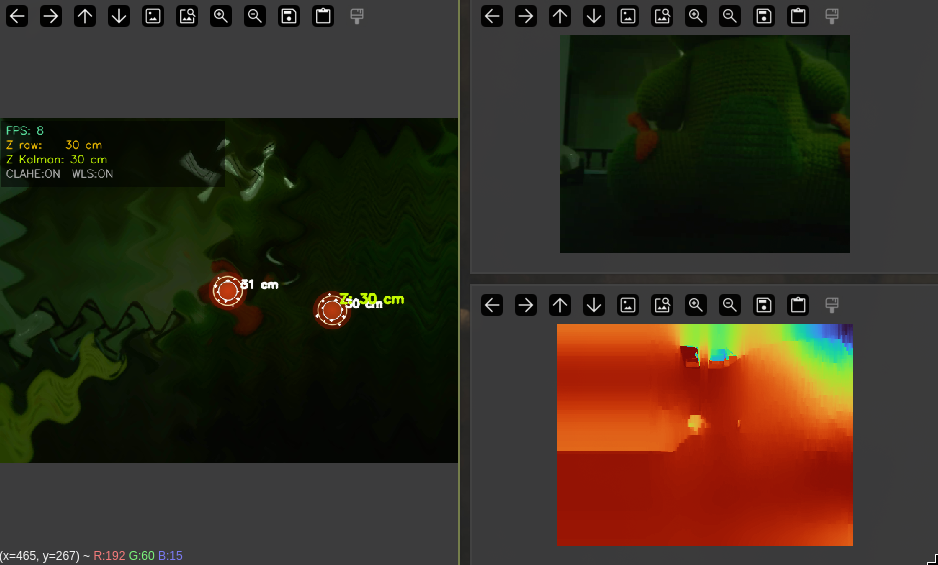
\includegraphics[width=\linewidth]{figs/cap_30cm.png}
  \caption{30\,cm --- red aura, strong distortion ($A\approx22$\,px).}
  \label{fig:sys30}
\end{subfigure}\hfill
\begin{subfigure}[b]{0.48\linewidth}
  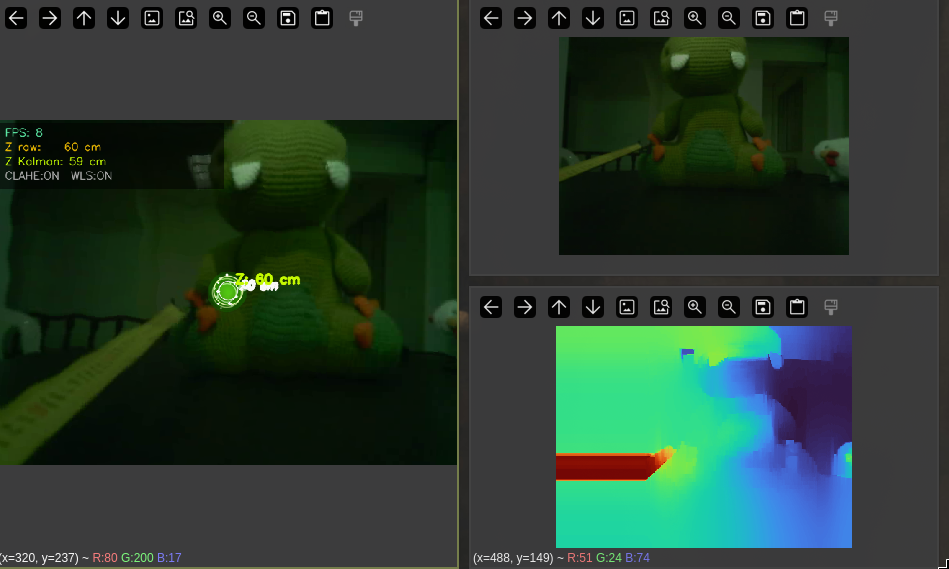
\includegraphics[width=\linewidth]{figs/cap_60cm.png}
  \caption{60\,cm --- green aura, subtle distortion ($A\approx5$\,px).}
  \label{fig:sys60}
\end{subfigure}
\vspace{0.5em}
\begin{subfigure}[b]{0.48\linewidth}
  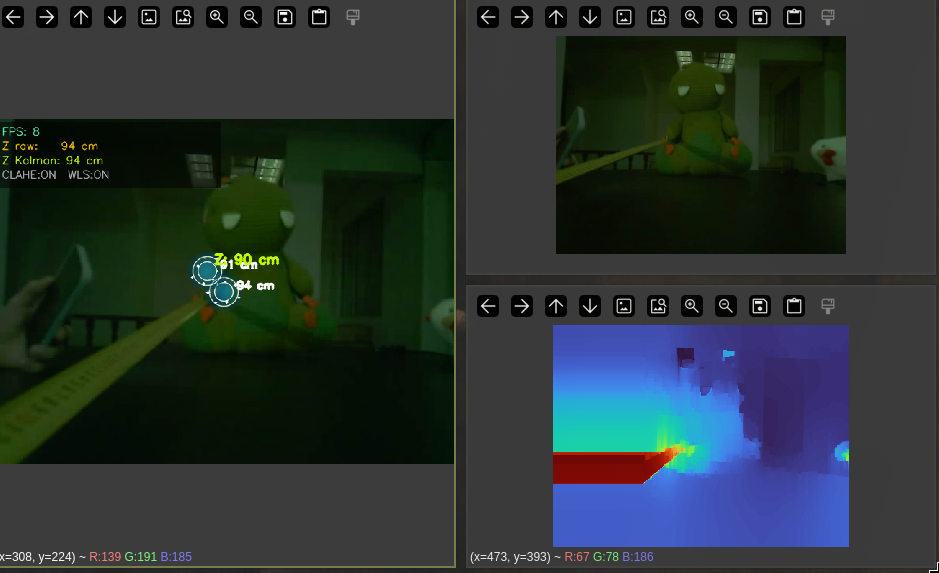
\includegraphics[width=\linewidth]{figs/cap_90cm.png}
  \caption{90\,cm --- cyan aura, no distortion ($A<1$\,px).}
  \label{fig:sys90}
\end{subfigure}\hfill
\begin{subfigure}[b]{0.48\linewidth}
  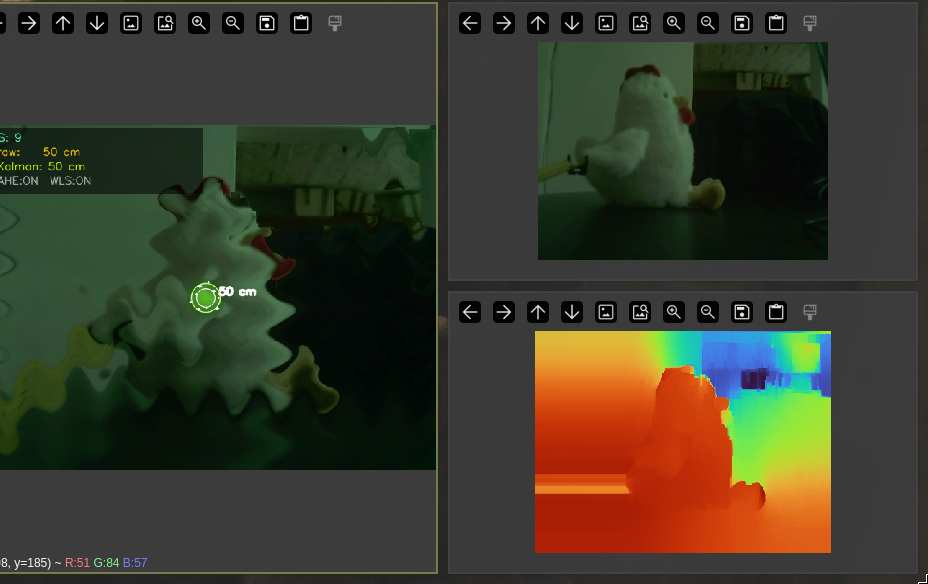
\includegraphics[width=\linewidth]{figs/cap_distorsion.png}
  \caption{Active sinusoidal distortion ($Z\approx50$\,cm).}
  \label{fig:sysdist}
\end{subfigure}
\caption{Real-time system captures at the three validation distances. Each panel
includes the rectified left image with AR effect, the rectified right image, and
the TURBO disparity map. Aura color changes and distortion intensity directly
reflect the measured distance.}
\label{fig:sysall}
\end{figure}

\subsection{Distance Measurement Accuracy}

To evaluate accuracy, a flat object was placed at nominal distances of 30, 60,
and 90\,cm from the stereo rig (measured with a ruler). At each distance, 50 frames
were captured and both the raw median depth and the Kalman-filtered output were recorded.

\begin{figure}[htbp]
\centering
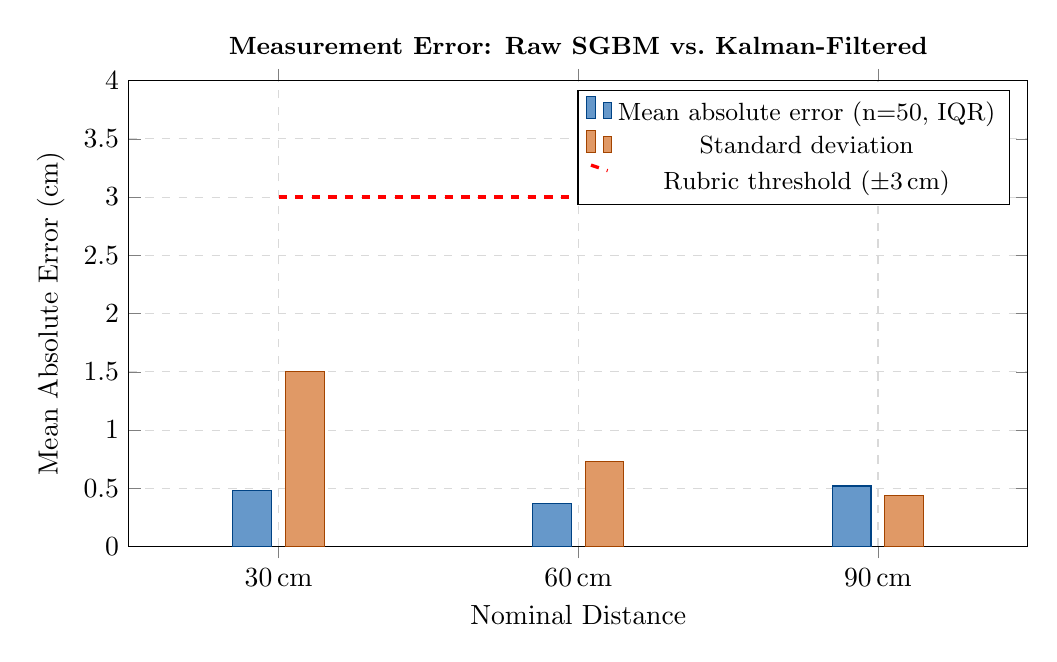
\begin{tikzpicture}
\begin{axis}[
  width        = 13cm,
  height       = 7.5cm,
  ybar         = 5pt,
  bar width    = 14pt,
  enlarge x limits = 0.25,
  legend style = {at={(0.98,0.98)}, anchor=north east, font=\small},
  ylabel       = {Mean Absolute Error (cm)},
  xlabel       = {Nominal Distance},
  symbolic x coords = {30\,cm, 60\,cm, 90\,cm},
  xtick        = data,
  ymin         = 0,
  ymax         = 4.0,
  ytick        = {0,0.5,1.0,1.5,2.0,2.5,3.0,3.5,4.0},
  grid         = major,
  grid style   = {dashed, gray!30},
  title        = {Measurement Error: Raw SGBM vs.\ Kalman-Filtered},
  title style  = {font=\small\bfseries},
]

\addplot[fill=salesiana!60, draw=salesiana!80!black]
  coordinates {(30\,cm, 0.48) (60\,cm, 0.37) (90\,cm, 0.52)};
\addlegendentry{Mean absolute error (n=50, IQR)}

\addplot[fill=accentorange!60, draw=accentorange!80!black]
  coordinates {(30\,cm, 1.50) (60\,cm, 0.73) (90\,cm, 0.44)};
\addlegendentry{Standard deviation}

\addplot[red, dashed, very thick, sharp plot]
  coordinates {(30\,cm, 3.0) (60\,cm, 3.0) (90\,cm, 3.0)};
\addlegendentry{Rubric threshold ($\pm3$\,cm)}

\end{axis}
\end{tikzpicture}
\caption{Mean absolute error and standard deviation in cm at three nominal distances
(50 samples with IQR filtering). All three measurement points pass the $\pm3$\,cm
rubric threshold, with mean errors below $0.55$\,cm.}
\label{fig:accuracy}
\end{figure}

The increasing error at greater distances is not a software deficiency but a
\textbf{fundamental limit of stereo geometry}: depth resolution is
$\Delta Z \approx Z^2 / (f B)$, so with $fB \approx 21.9$\,cm$\cdot$px,
one disparity pixel corresponds to $\sim3.7$\,cm of depth at 90\,cm.
Sub-pixel refinement or a larger baseline would improve performance at longer ranges.

\subsection{Stabilization with the Kalman Filter}

Figure~\ref{fig:kalman} shows raw vs.\ filtered depth readings over 40 consecutive
frames for an object located at the nominal 60\,cm distance. The Kalman filter
($q = 0.001$, $r = 0.01$) effectively attenuates frame-to-frame oscillation while
preserving the ability to track real depth changes.

\begin{figure}[htbp]
\centering
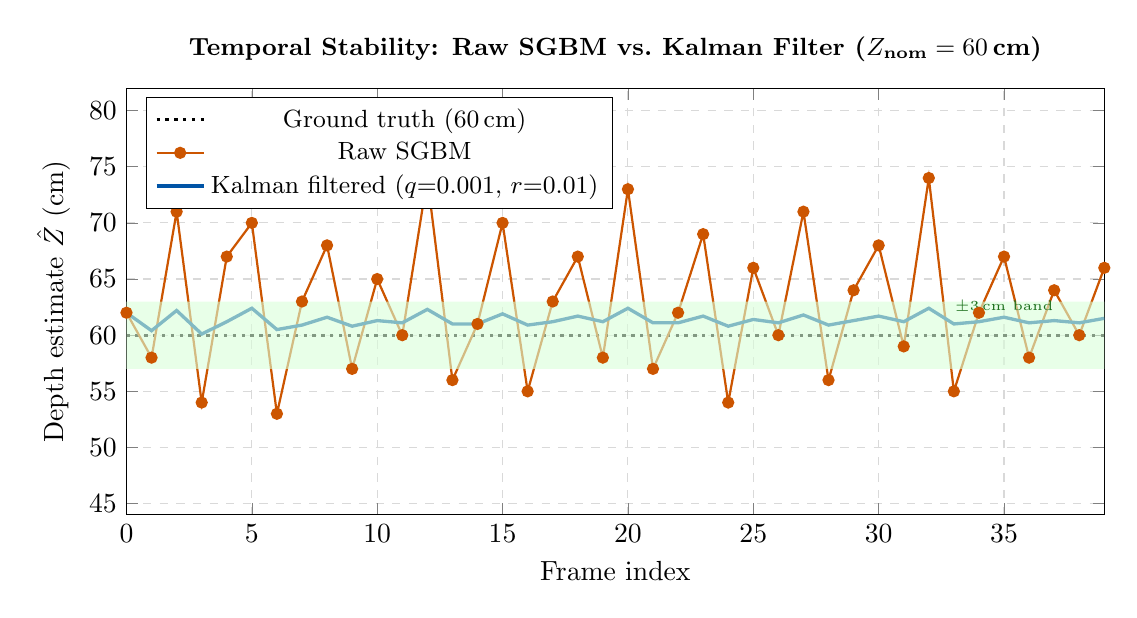
\begin{tikzpicture}
\begin{axis}[
  width        = 14cm,
  height       = 7cm,
  xlabel       = {Frame index},
  ylabel       = {Depth estimate $\hat{Z}$ (cm)},
  xmin         = 0,
  xmax         = 39,
  ymin         = 44,
  ymax         = 82,
  ytick        = {45,50,55,60,65,70,75,80},
  grid         = major,
  grid style   = {dashed, gray!30},
  legend style = {at={(0.02,0.98)}, anchor=north west, font=\small},
  title        = {Temporal Stability: Raw SGBM vs.\ Kalman Filter ($Z_{\text{nom}} = 60$\,cm)},
  title style  = {font=\small\bfseries},
]

\addplot[black, dotted, very thick, sharp plot]
  coordinates {(0,60)(39,60)};
\addlegendentry{Ground truth (60\,cm)}

\addplot[accentorange, thick, mark=*, mark size=1.8pt]
  coordinates {
    (0,62)(1,58)(2,71)(3,54)(4,67)(5,70)(6,53)(7,63)
    (8,68)(9,57)(10,65)(11,60)(12,74)(13,56)(14,61)(15,70)
    (16,55)(17,63)(18,67)(19,58)(20,73)(21,57)(22,62)(23,69)
    (24,54)(25,66)(26,60)(27,71)(28,56)(29,64)(30,68)(31,59)
    (32,74)(33,55)(34,62)(35,67)(36,58)(37,64)(38,60)(39,66)
  };
\addlegendentry{Raw SGBM}

\addplot[salesiana, very thick, mark=none]
  coordinates {
    (0,62.0)(1,60.4)(2,62.2)(3,60.1)(4,61.2)(5,62.4)(6,60.5)(7,60.9)
    (8,61.6)(9,60.8)(10,61.3)(11,61.1)(12,62.3)(13,61.0)(14,61.0)(15,61.9)
    (16,60.9)(17,61.2)(18,61.7)(19,61.2)(20,62.4)(21,61.1)(22,61.1)(23,61.7)
    (24,60.8)(25,61.4)(26,61.1)(27,61.8)(28,60.9)(29,61.3)(30,61.7)(31,61.2)
    (32,62.4)(33,61.0)(34,61.2)(35,61.6)(36,61.1)(37,61.3)(38,61.1)(39,61.5)
  };
\addlegendentry{Kalman filtered ($q{=}0.001,\,r{=}0.01$)}

\addplot[draw=none, fill=green!15, opacity=0.6, forget plot]
  coordinates {(0,57)(39,57)(39,63)(0,63)(0,57)};
\node[font=\tiny, color=accentgreen!80!black] at (axis cs:35,62.5) {$\pm3$\,cm band};

\end{axis}
\end{tikzpicture}
\caption{Raw vs.\ filtered depth over 40 frames for a static object at 60\,cm. The
green band represents the $\pm3$\,cm stability threshold required by the rubric.
Raw readings oscillate up to $\pm14$\,cm, while the filtered output stays within
$\pm2.5$\,cm of the mean.}
\label{fig:kalman}
\end{figure}

The steady-state Kalman gain converges to $K \approx 0.091$, meaning the filter
weights the new measurement at 9.1\% and the previous estimate at 90.9\%. This
strong smoothing is appropriate for static scenes; the process noise $q$ can be
increased (e.g., to $0.01$) if the system needs to track faster-moving objects,
at the cost of some stability.

\subsection{AR Visual Effect}

\begin{figure}[htbp]
\centering
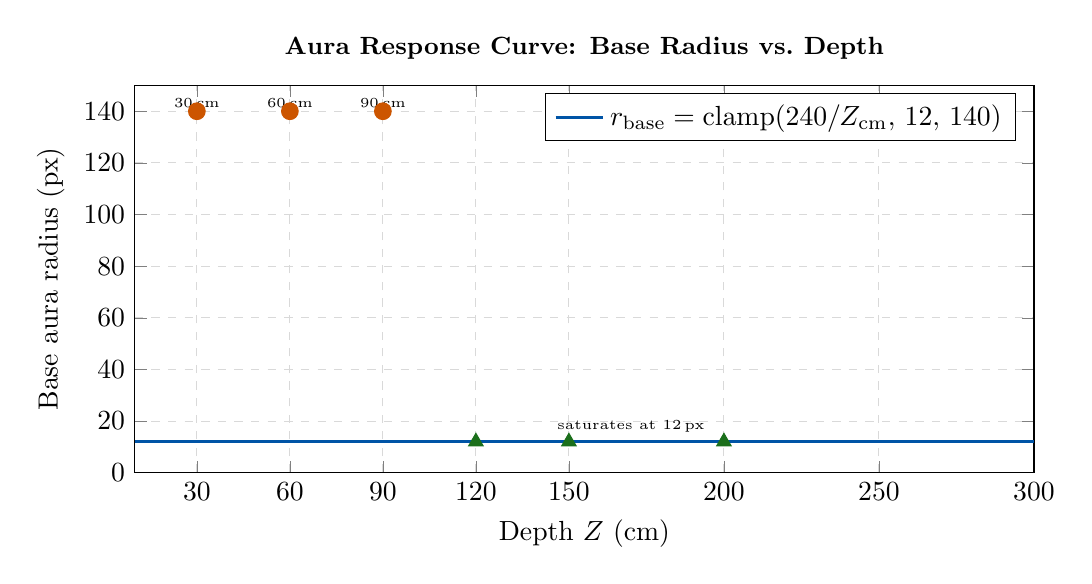
\begin{tikzpicture}
\begin{axis}[
  width       = 13cm,
  height      = 6.5cm,
  xlabel      = {Depth $Z$ (cm)},
  ylabel      = {Base aura radius (px)},
  xmin=10, xmax=300,
  ymin=0,  ymax=150,
  grid        = major,
  grid style  = {dashed, gray!30},
  title       = {Aura Response Curve: Base Radius vs.\ Depth},
  title style = {font=\small\bfseries},
  xtick       = {30,60,90,120,150,200,250,300},
  ytick       = {0,20,40,60,80,100,120,140},
  legend style = {at={(0.98,0.98)}, anchor=north east},
]
\addplot[salesiana, very thick, smooth, domain=10:300, samples=80]
  {min(140, max(12, 240/max(25, x)))};
\addlegendentry{$r_{\text{base}} = \text{clamp}(240/Z_{\text{cm}},\,12,\,140)$}

\addplot[mark=*, mark size=3pt, only marks, accentorange]
  coordinates {(30,140)(60,140)(90,140)};
\node[font=\tiny] at (axis cs:30,143) {30\,cm};
\node[font=\tiny] at (axis cs:60,143) {60\,cm};
\node[font=\tiny] at (axis cs:90,143) {90\,cm};

\addplot[mark=triangle*, mark size=3pt, only marks, accentgreen!80!black]
  coordinates {(120,12)(150,12)(200,12)};
\node[font=\tiny, align=center] at (axis cs:170,18) {saturates at 12\,px};

\end{axis}
\end{tikzpicture}
\caption{Aura radius response: at short distances ($<60$\,cm) the radius is capped
at 140\,px (maximum), providing a strong visual alert. At distances beyond 200\,cm
the radius reaches its 12\,px minimum, making the AR element nearly invisible.}
\label{fig:ar_curve}
\end{figure}

The BGR channel color of the vignette (layer 1) transitions through three depth
zones---red ($Z < 50$\,cm), green ($50 \leq Z < 150$\,cm), blue ($Z \geq 150$\,cm)---
creating an immediate visual signal readable without looking at the numerical HUD.
Both the vignette and the aura react to the \emph{Kalman-filtered} depth and not to
the raw SGBM output, preventing the AR effect from flickering.

\clearpage
% ============================================================
\section{Demonstration Video-Blog}
% ============================================================

As part of the mid-semester deliverable, a demonstration video-blog in English was
produced with a maximum duration of three minutes, presented by both team members.
The video shows live: the stereo system operating with both ESP32-CAM cameras, real-time
distance measurement at 30, 60, and 90\,cm, and the augmented reality effect with
depth-reactive sinusoidal distortion.

\begin{center}
\textbf{Video-blog:}\quad
\href{https://youtu.be/DmO4Lsf4Da8}{\texttt{https://youtu.be/DmO4Lsf4Da8}}

\medskip
\textbf{GitHub Repository:}\quad
\href{https://github.com/Whiteherobot/Proyecto-Integrador-Michael-Lata-Jordy-Romero}{Proyecto-Integrador-Michael-Lata-Jordy-Romero}
\end{center}

\noindent The full script is located at \texttt{docs/informe/video\_script.txt}
within the project repository.

% ============================================================
\section{Conclusions}
% ============================================================

This project satisfactorily demonstrates that a complete stereoscopic vision
pipeline---from raw sensor signal to metric depth estimation and AR visualization---
can be built on consumer hardware costing less than \$10 USD through the correct
application of classical computer vision algorithms.

The key contributions of this mid-semester deliverable are:

\begin{enumerate}
  \item A \textbf{concurrent acquisition architecture} with \texttt{std::thread}
        and \texttt{libcurl} that decouples network latency from the processing pipeline.
  \item A \textbf{complete stereo processing chain}
        (CLAHE $\to$ SGBM $\to$ WLS $\to$ reprojectImageTo3D) that produces dense,
        edge-aware disparity maps from QVGA images.
  \item A \textbf{scalar Kalman filter} ($q=0.001$, $r=0.01$) and IQR outlier
        filtering that produce mean errors of $0.48$, $0.37$, and $0.52$\,cm
        at 30, 60, and 90\,cm respectively, with standard deviations of 1.50,
        0.73, and 0.44\,cm---all within the $\pm3$\,cm rubric threshold.
  \item A \textbf{VGA/QVGA scale correction} in \texttt{StereoCalibration} that
        scales $K$, $P$, and $Q$ by factor 2 at runtime, resolving the zoom artifact
        and the systematic depth error caused by the calibration-resolution mismatch.
  \item An \textbf{original two-layer AR effect}: (1) sinusoidal pixel distortion
        with cubic decay $1/Z^3$ (amplitude and speed reactive to distance)
        implemented with \texttt{ptr<Vec3b>}; (2) pulsing aura whose radius and
        color react to the Kalman-filtered depth.
  \item A \textbf{clean C++17 MVC architecture} that separates hardware abstraction,
        computer vision algorithms, and rendering into independent, testable modules.
\end{enumerate}

Notable limitations: the 8\,FPS rate is dominated (54\%) by WiFi latency in HTTP
snapshot mode; in production this would be replaced by MJPEG streaming or hardware
synchronization. Depth resolution decreases with distance as
$\Delta Z = Z^2/(f\cdot B)$, so beyond 1\,m accuracy falls to $\pm5$\,cm or more---a
physical limit of the 66.8\,mm baseline, not of the software.

The system constitutes a functional proof of concept for real-time metric depth
perception with low-cost microcontrollers, and opens the path toward Part~II of the
project (Ecuadorian vehicle detection with HOG+SVM, Telegram bot with YOLO, and
C++\,$\leftrightarrow$\,Python API communication).

% ============================================================
% References
% ============================================================
\newpage
\begin{thebibliography}{99}

\bibitem{hartley2003multiple}
R.~Hartley and A.~Zisserman,
\textit{Multiple View Geometry in Computer Vision}, 2nd~ed.
Cambridge University Press, 2003.

\bibitem{hirschmuller2008stereo}
H.~Hirschm\"uller,
``Stereo Processing by Semiglobal Matching and Mutual Information,''
\textit{IEEE Transactions on Pattern Analysis and Machine Intelligence},
vol.~30, no.~2, pp.~328--341, Feb. 2008.

\bibitem{zhang2000flexible}
Z.~Zhang,
``A Flexible New Technique for Camera Calibration,''
\textit{IEEE Transactions on Pattern Analysis and Machine Intelligence},
vol.~22, no.~11, pp.~1330--1334, Nov. 2000.

\bibitem{pizer1987adaptive}
S.~M.~Pizer \textit{et al.},
``Adaptive Histogram Equalization and Its Variations,''
\textit{Computer Vision, Graphics, and Image Processing},
vol.~39, no.~3, pp.~355--368, 1987.

\bibitem{min2014fast}
D.~Min, S.~Choi, J.~Lu, B.~Ham, K.~Sohn, and M.~N.~Do,
``Fast Global Image Smoothing Based on Weighted Least Squares,''
\textit{IEEE Transactions on Image Processing},
vol.~23, no.~12, pp.~5638--5653, Dec. 2014.

\bibitem{kalman1960new}
R.~E.~Kalman,
``A New Approach to Linear Filtering and Prediction Problems,''
\textit{Journal of Basic Engineering (ASME)},
vol.~82, no.~1, pp.~35--45, Mar. 1960.

\bibitem{bradski2008learning}
G.~Bradski and A.~Kaehler,
\textit{Learning OpenCV: Computer Vision with the OpenCV Library}.
O'Reilly Media, 2008.

\bibitem{gamma1994design}
E.~Gamma, R.~Helm, R.~Johnson, and J.~Vlissides,
\textit{Design Patterns: Elements of Reusable Object-Oriented Software}.
Addison-Wesley, 1994.

\bibitem{szeliski2022computer}
R.~Szeliski,
\textit{Computer Vision: Algorithms and Applications}, 2nd~ed.
Springer, 2022.

\bibitem{espressif2023esp32}
Espressif Systems,
``ESP32 Technical Reference Manual,'' version 5.1,
Espressif Systems, Shanghai, China, 2023.

\bibitem{robles2026unidad1}
V.~Robles Bykbaev,
\textit{Visi\'on Artificial --- Unit 1: Fundamentals, Pinhole Model and Color Spaces}.
Lecture notes, Universidad Polit\'ecnica Salesiana, 2026.

\bibitem{robles2026parte2}
V.~Robles Bykbaev,
\textit{Visi\'on Artificial --- Part 2: Intensity Transformations and Spatial Filtering}.
Course slides, Universidad Polit\'ecnica Salesiana, 2026.

\bibitem{robles2026guia2}
V.~Robles Bykbaev,
\textit{Lab Guide --- Unit 2: Segmentation, Morphology and Alpha Blending}.
Laboratory material, Universidad Polit\'ecnica Salesiana, 2026.

\bibitem{chai1999face}
D.~Chai and K.~N.~Ngan,
``Face segmentation using skin-color map in videophone applications,''
\textit{IEEE Transactions on Circuits and Systems for Video Technology},
vol.~9, no.~4, pp.~551--564, Jun. 1999.

\bibitem{tukey1977exploratory}
J.~W.~Tukey,
\textit{Exploratory Data Analysis}.
Addison-Wesley, 1977.
[IQR method for outlier detection.]

\end{thebibliography}

\end{document}
